\documentclass[a4paper]{article}

\usepackage{fullpage} % Package to use full page
\usepackage{parskip} % Package to tweak paragraph skipping
\usepackage{amsmath}
\usepackage{amssymb}
\usepackage{hyperref}
\usepackage{subcaption}
\usepackage{graphicx}
\usepackage{fancyvrb}

\title{16-720B Computer Vision: Homework 4 \\
3D Reconstruction}
\author{Heethesh Vhavle\\
Andrew ID: hvhavlen}
\date{11 November 2018\\(Using \textbf{TWO LATE DAYS})}

\begin{document}

\maketitle

\section{Theory}
\subsection{}
It is given that the principal axes for both cameras intersect at the point P. Thus, they are corresponding points and we have the following relation when the points are at the origins.
\begin{gather}
\begin{array}{c}
    \boldsymbol{x _ { 2 } ^ { T } F x} _ { 1 } = 0
    &  \\
    \left[ \begin{array} { l l l } { x _ { 2 } } & { y _ { 2 } } & { 1 } \end{array} \right] \left[ \begin{array} { l l l } { F _ { 11 } } & { F _ { 12 } } & { F _ { 13 } } \\ { F _ { 21 } } & { F _ { 22 } } & { F _ { 23 } } \\ { F _ { 31 } } & { F _ { 32 } } & { F _ { 33 } } \end{array} \right] \left[ \begin{array} { c } { x _ { 1 } } \\ { y _ { 1 } } \\ { 1 } \end{array} \right] = 0
    & \\
    \left[ \begin{array} { l l l } { 0 } & { 0 } & { 1 } \end{array} \right] \left[ \begin{array} { l l l } { F _ { 11 } } & { F _ { 12 } } & { F _ { 13 } } \\ { F _ { 21 } } & { F _ { 22 } } & { F _ { 23 } } \\ { F _ { 31 } } & { F _ { 32 } } & { F _ { 33 } } \end{array} \right] \left[ \begin{array} { c } { 0 } \\ { 0 } \\ { 1 } \end{array} \right] = 0
\end{array}
\end{gather}

On simplifying this, all the terms that have the image point coordinates get cancelled at the origin and therefore, we have the following relation.
\begin{gather}
    F _ { 33 } = 0
\end{gather}

\subsection{}
For pure translation along the x-axis, we have the following transformation matrices.
\begin{gather}
\begin{array}{c}
    \boldsymbol { R } = \left[ \begin{array} { l l l } { 1 } & { 0 } & { 0 } \\ { 0 } & { 1 } & { 0 } \\ { 0 } & { 0 } & { 1 } \end{array} \right]
    &  \\
    \boldsymbol{t} = \left[ \begin{array} { l } { t _ { 1 } } \\ { 0 } \\ { 0 } \end{array} \right]
\end{array}
\end{gather}

We also know the following relation for an essential matrix.
\begin{gather}
    \mathbf { E } = \mathbf { t _ {\times} } \mathbf { R }
\end{gather}

We can write $\mathbf { t _ {\times} }$ as follows and obtain the essential matrix.
\begin{gather}
\begin{array}{c}
    \mathbf { t _ {\times} } = \left[ \begin{array} { c c c } { 0 } & { 0 } & { 0 } \\ { 0 } & { 0 } & { - t _ { 1 } } \\ { 0 } & { t _ { 1 } } & { 0 } \end{array} \right]
    & \\
    \mathbf { E } = \left[ \begin{array} { c c c } { 0 } & { 0 } & { 0 } \\ { 0 } & { 0 } & { - t _ { 1 } } \\ { 0 } & { t _ { 1 } } & { 0 } \end{array} \right]
\end{array}
\end{gather}

Now, for any given point in image 1, we have an epipolar line in image plane 2.
\begin{gather}
    \begin{array}{c}
        \boldsymbol{l _ { 2 }} = \mathbf{E} \boldsymbol{x _ { 1 } }
        &  \\
        \boldsymbol{l _ { 2 }} = \left[ \begin{array} { c c c } { 0 } & { 0 } & { 0 } \\ { 0 } & { 0 } & { - t _ { 1 } } \\ { 0 } & { t _ { 1 } } & { 0 } \end{array} \right] \left[ \begin{array} { c } { x _ { 1 } } \\ { y _ { 1 } } \\ { 1 } \end{array} \right]
        & \\
        \boldsymbol{l _ { 2 }} = \left[ \begin{array} { c } { 0 } \\ { - t _ { 1 } } \\ { y _ { 1 } } \end{array} \right]
    \end{array}
\end{gather}

We can rewrite the above in the line equation form as follows for image 2.
\begin{gather}
    { y_{2} } = { y_{1} }
\end{gather}

Therefore, this is a line parallel to the x-axis in image 2 and similarly, it can be shown that the epipolar line in image 1 is also parallel to the x-axis for a point in image 2.

\subsection{}
We can use the concept of composition of homogeneous transformations to solve this problem. We know the following transformations with respect to the inertial frames, measured by the sensors.
\begin{gather}
    \begin{array}{c}
        \mathbf{ { H_{1}^{0} } } = [ \mathbf { R_{1} } | \mathbf { t_{1} } ]
        &  \\
        \mathbf{ { H_{2}^{0} } } = [ \mathbf { R_{2} } | \mathbf { t_{2} } ]
    \end{array}
\end{gather}

The relative transformation,
\begin{gather}
    \begin{array}{c}
    \mathbf{ { H_{2}^{1} } } = [ \mathbf { R_{rel} } | \mathbf { t_{rel} } ]
    & \\
    \mathbf{ { H_{2}^{1} } } = \left( \mathbf{ H _ { 1 } ^ { 0 } } \right) ^ { - 1 } \mathbf{ { H_{2}^{0} } }
    & \\
    \mathbf{ { H_{2}^{1} } } = \left[ \begin{array} { c c } { \mathbf{R _ { 1 } ^ { T }}  } & { \mathbf{-R _ { 1 } ^ { T }} \mathbf{t _ { 1 }} } \\ { \mathbf{0} } & { 1 } \end{array} \right] \left[ \begin{array} { c c } { \mathbf{R _ { 2 }} } & { \mathbf{t _ { 2 }} } \\ { \mathbf{0} } & { 1 } \end{array} \right]
    & \\
    \mathbf{ { H_{2}^{1} } } = \left[ \begin{array} { c c } { \mathbf{R _ { 1 } ^ { T }} \mathbf{R _ { 2 }} } & { \mathbf{R _ { 1 } ^ { T }} \mathbf{t _ { 2 }} \mathbf{-R _ { 1 } ^ { T }} \mathbf{t _ { 1 }} } \\ { \mathbf{0} } & { 1 } \end{array} \right]
    & \\
    \mathbf { R_{rel} } = \mathbf{R _ { 1 } ^ { T }} \mathbf{R _ { 2 }}
    & \\
    \mathbf { t_{rel} } = \mathbf{R _ { 1 } ^ { T }} (\mathbf{t _ { 2 }} - \mathbf{t _ { 1 }})
    \end{array}
\end{gather}

We can now use the known relations for the essential and fundamental matrices.
\begin{gather}
\begin{array}{c}
    \mathbf { E } = \mathbf { t _ {\times rel} } \mathbf { R_{rel} }
    &  \\
    \mathbf { F } = \mathbf { K ^ {-T} } \mathbf { E } \mathbf { K }
    & \\
    \mathbf { F } = \mathbf { K ^ {-T} } \mathbf { t _ {\times rel} } \mathbf { R_{rel} } \mathbf { K }
\end{array}
\end{gather}

\subsection{}
Let $C$ be the camera in the real world and $C^{\prime}$ be the camera in the virtual world and $\boldsymbol{K}$ be the intrinsic matrix for both the cameras. Let $\mathbf{P}$ and $\mathbf{x}$ be the 3D point in real world and the point in image plane and $\mathbf{P^{\prime}}$ and $\mathbf{x^{\prime}}$ be its reflection in the in the mirror and this point in the image plane. Given the mirror is flat, the transformation between these two points is a pure translation.
\begin{gather}
\begin{array}{c}
    \boldsymbol { R } = \left[ \begin{array} { l l l } { 1 } & { 0 } & { 0 } \\ { 0 } & { 1 } & { 0 } \\ { 0 } & { 0 } & { 1 } \end{array} \right]
    & \\
    \boldsymbol{t} = \left[ \begin{array} { l } { t _ { 1 } } \\ { t _ { 2 } } \\ { t _ { 3 } } \end{array} \right]
    & \\
    \mathbf{P^{\prime}} = \mathbf{P} + \mathbf{t}
    & \\
    \lambda _ { 1 } \mathbf{x} = K \mathbf{P}
    & \\
    \lambda _ { 2 } \mathbf{x^{\prime}} = K \mathbf{P^{\prime}}
\end{array}
\end{gather}

Using the above equations, we can now write the relationship between the two points as follows.
\begin{gather}
    \lambda _ { 2 } K ^ { - 1 } \mathbf{x^{\prime}} = \lambda _ { 1 } K ^ { - 1 } \mathbf{x} + \mathbf{t}
\end{gather}

We can simplify the equation and eliminate some terms by taking cross product with $\mathbf{t}$ on both sides, followed by dot product with $\mathbf{x^{\prime}}$ to get the following.
\begin{gather}
\begin{array}{c}
    \mathbf{x^{\prime}} ^ { T } K ^ { - T } \mathbf{t_{\times}} K ^ { - 1 } \mathbf{x} = 0
    &  \\
    \mathbf { t _ {\times} } = \left[ \begin{array} { c c c } { 0 } & { -t _ { 3 } } & { t _ { 2 } } \\ { t _ { 3 } } & { 0 } & { - t _ { 1 } } \\ { -t _ { 2 } } & { t _ { 1 } } & { 0 } \end{array} \right]
\end{array}
\end{gather}

We can see that, $\mathbf { t _ {\times} }$ is a skew-symmetric matrix here and we know the relation that $\mathbf{x^{\prime}} ^ { T }\mathbf{F}\mathbf{x}=0$. Comparing this with above form, we get the following expression for \textbf{F}.
\begin{gather}
    \mathbf{F} = K ^ { - T } \mathbf{t_{\times}} K ^ { - 1 }
\end{gather}

Since, $\mathbf { t _ {\times} }$ is skew symmetric, it can be shown that \textbf{F} here will also retain the property of skew-symmetric for a given intrinsic matrix \textbf{K}.
\begin{gather}
    \mathbf{F ^ { T }} = -\mathbf{F}
\end{gather}

Therefore, we can conclude that the two images of the object are related by a skew-symmetric fundamental matrix.

\section{Fundamental Matrix Estimation}
\subsection{The Eight Point Algorithm}
\begin{figure}[!ht]
\centering
\begin{tabular}{c}
{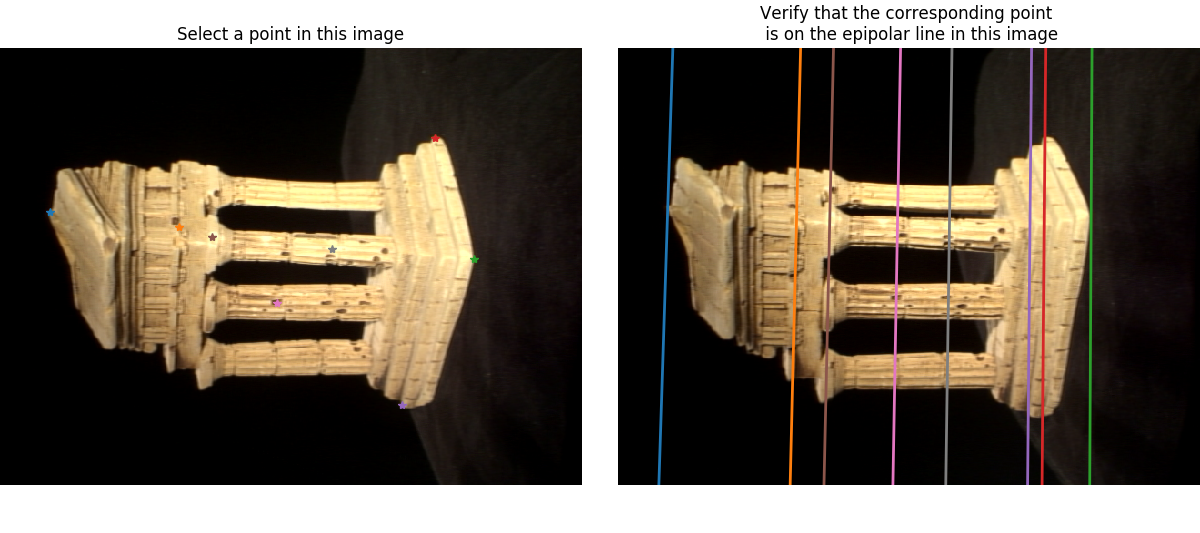
\includegraphics[width=\textwidth]{images/eightpoint.png}}
\end{tabular}
\caption{Eight-Point Algorithm Output}
\end{figure}

\begin{figure}[!ht]
\centering
\begin{BVerbatim}
[[-8.33149231e-09  1.29538462e-07 -1.17187851e-03]
 [ 6.51358337e-08  5.70670060e-09 -4.13435037e-05]
 [ 1.13078765e-03  1.91823637e-05  4.16862080e-03]]
\end{BVerbatim}
\caption{Fundamental Matrix recovered from Eight-Point Algorithm}
\end{figure}

\subsection{The Seven Point Algorithm}
\begin{figure}[!ht]
\centering
\begin{tabular}{c}
{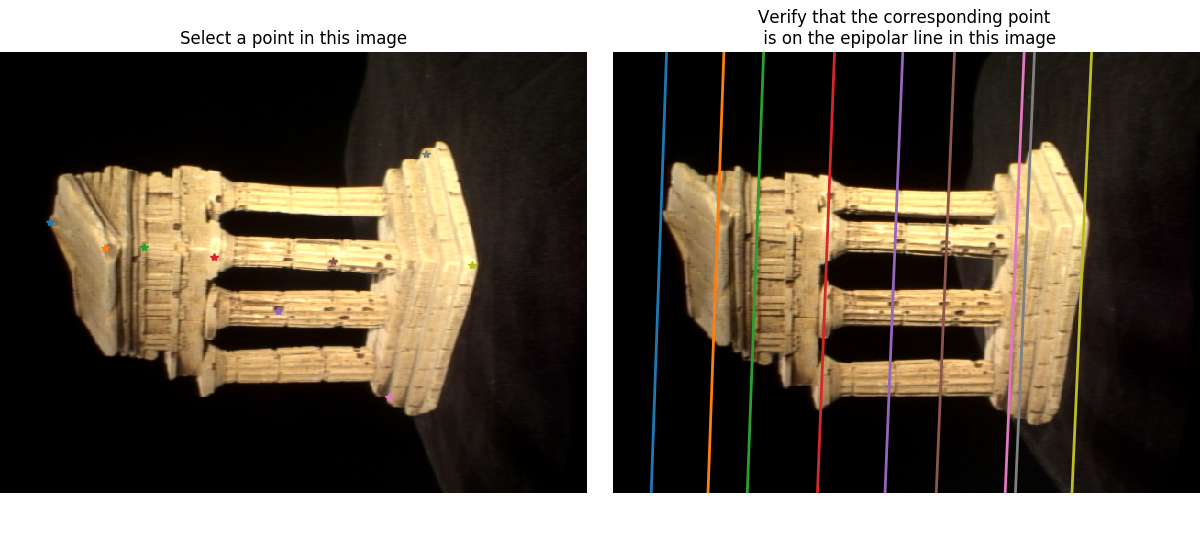
\includegraphics[width=\textwidth]{images/sevenpoint.png}}
\end{tabular}
\caption{Seven-Point Algorithm Output}
\end{figure}

The \textbf{third fundamental matrix} from the recovered set was found to be the correct one and is used for the visualization.

\begin{figure}[!ht]
\centering
\begin{BVerbatim}
[[-1.29112668e-06,  7.07910920e-06, -2.66910095e-03],
 [-6.12061099e-06,  2.62897062e-06, -5.54238146e-04],
 [ 3.08512019e-03, -8.26588573e-04,  8.43474773e-02]]

[[ 6.90594357e-07, -3.95406822e-06,  1.83830500e-04],
 [ 3.70536589e-06, -1.59312872e-06,  2.89750890e-04],
 [-4.57898759e-04,  4.90784533e-04, -4.62403318e-02]]

[[-6.08872858e-08,  2.29785168e-07, -8.98019857e-04],
 [-2.07091188e-08,  7.91909582e-09, -3.02952995e-05],
 [ 8.85637310e-04, -8.77200649e-06,  3.27942364e-03]]
\end{BVerbatim}
\caption{Fundamental Matrices recovered from Seven-Point Algorithm}
\end{figure}

\section{Metric Reconstruction}
\subsection{Essential Matrix}
\begin{figure}[!ht]
\centering
\begin{BVerbatim}
[[-1.92592123e-02  3.00526429e-01 -1.73693252e+00]
 [ 1.51113725e-01  1.32873151e-02 -3.08885272e-02]
 [ 1.73986815e+00  9.11774761e-02  3.90697725e-04]]
\end{BVerbatim}
\caption{Estimated Essential Matrix}
\end{figure}

\subsection{Triangulation}
We have the following relationship for given 2D point and the corresponding 3D point for a camera matrix \textbf{C}.
\begin{gather}
\begin{array}{c}
    \tilde { \boldsymbol { x } } _ { i } = C \boldsymbol{{w}_{i}}
    & \\
    \tilde { \boldsymbol { x } } _ { i } \times C \boldsymbol{{w}_{i}} = 0
    & \\
    \left[ \begin{array} { l } { x } \\ { y } \\ { 1 } \end{array} \right] \times \left[ \begin{array} { c c c c } { C _ { 11 } } & { C _ { 12 } } & { C _ { 13 } } & { C _ { 14 } } \\ { C _ { 21 } } & { C _ { 22 } } & { C _ { 23 } } & { C _ { 24 } } \\ { C _ { 31 } } & { C _ { 32 } } & { C _ { 33 } } & { C _ { 34 } } \end{array} \right] \left[ \begin{array} { l } { X } \\ { Y } \\ { Z } \\ { 1 } \end{array} \right] = 0
\end{array}
\end{gather}
For the two cameras, we can write it in the following form with A matrix and solve for the 3D points using SVD.
\begin{gather}
\begin{array}{c}
    \boldsymbol{A_{i}} \boldsymbol{{w}_{i}} = \boldsymbol { 0 }
    &  \\
    \boldsymbol{A_{i}} = \left[ \begin{array} { c } { y _ { i1 } C _{1} ^ { 3 T } - C _{1} ^ { 2 T } } \\ { x _ { i1 } C _{1} ^ { 3 T } - C _{1} ^ { 1 T } } \\ { y _ { i2 } C _{2} ^ { 3 T } - C _{2} ^ { 2 T } } \\ { x _ { i2 } C _{2} ^ { 3 T } - C _{2} ^ { 1T } } \end{array} \right]
\end{array}
\end{gather}

\subsection{Finding M2}
The function has been implemented in \texttt{findM2.py}.

\section{3D Visualization}
\subsection{Epipolar Correspondences}
\begin{figure}[!ht]
\centering
\begin{tabular}{c}
{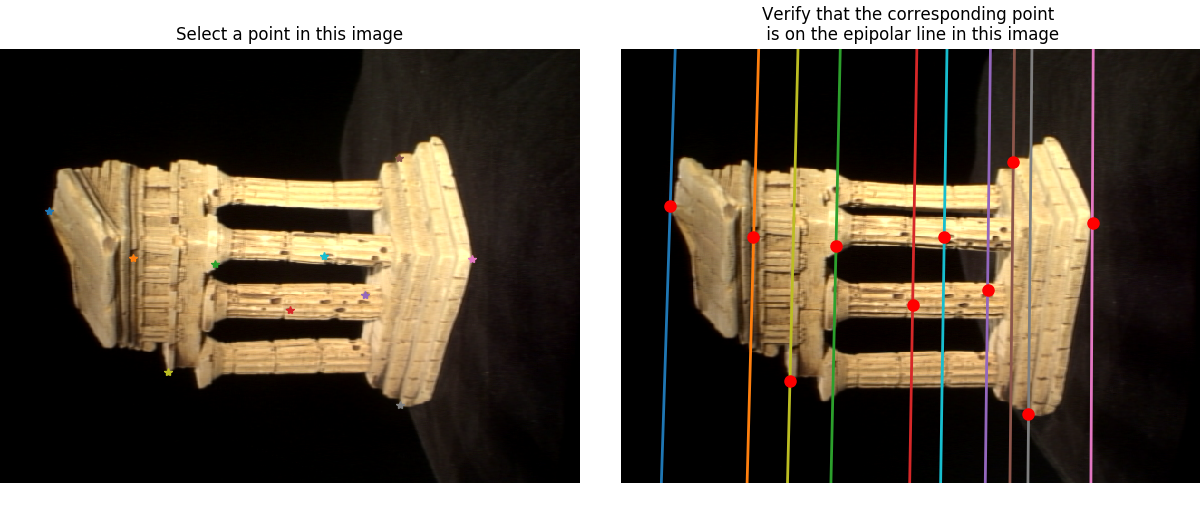
\includegraphics[width=\textwidth]{images/correspondences.png}}
\end{tabular}
\caption{Epipolar Correspondences}
\end{figure}

\subsection{Visualization}
\begin{figure}[!ht]
\centering
\begin{tabular}{ccc}
{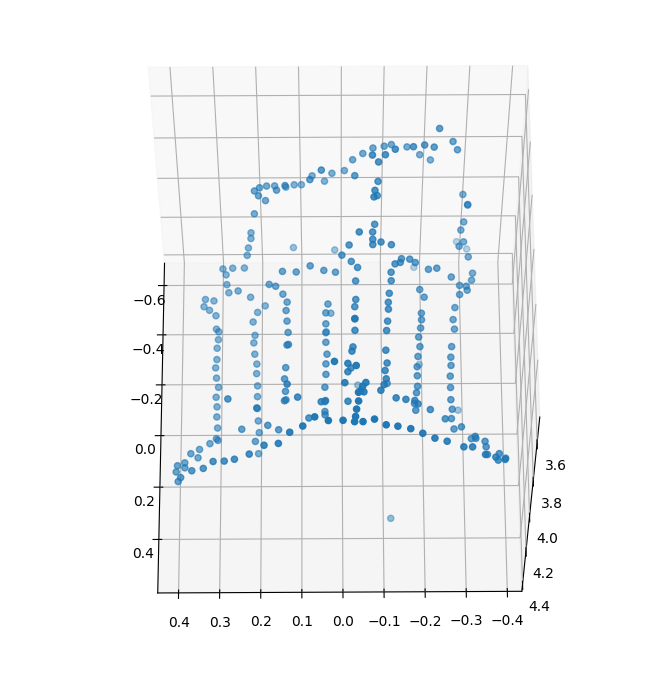
\includegraphics[width=0.3\textwidth]{images/temple1.png}} &
{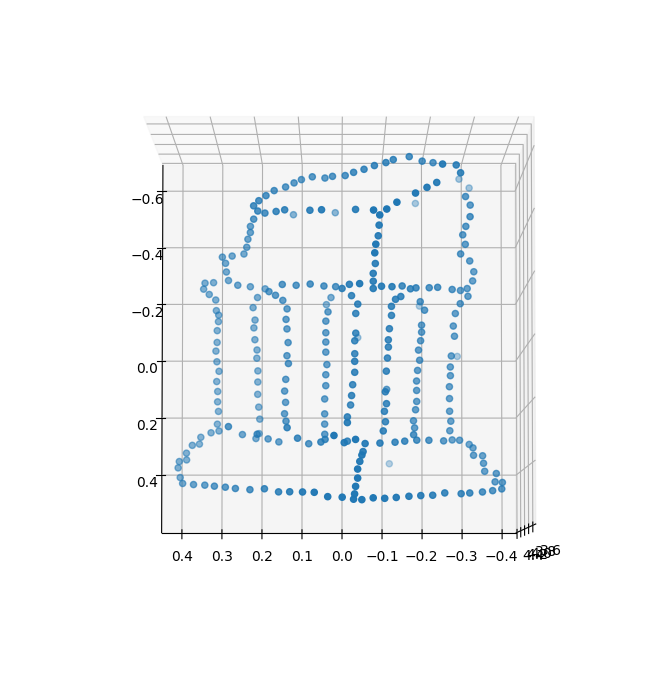
\includegraphics[width=0.3\textwidth]{images/temple2.png}} &
{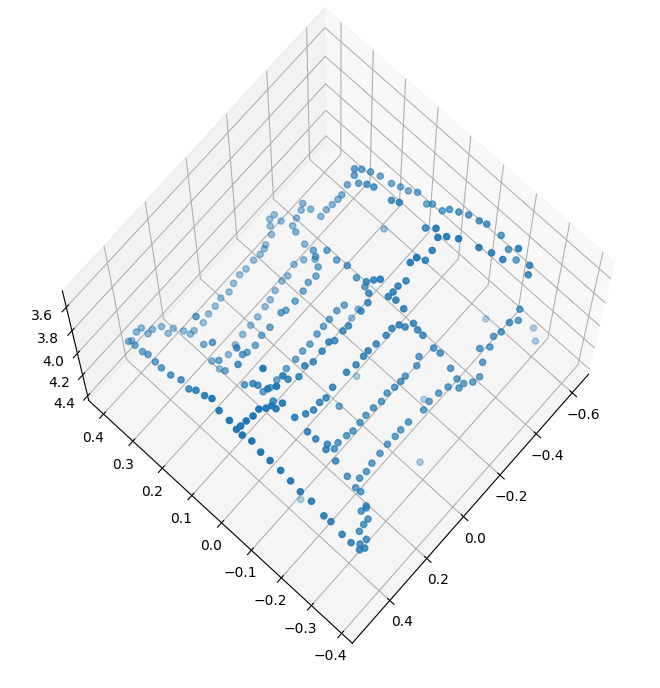
\includegraphics[width=0.3\textwidth]{images/temple3.png}}
\end{tabular}
\caption{3D Visualization of the Temple}
\end{figure}

\section{Bundle Adjustment}
\subsection{The Seven Point Algorithm with RANSAC}
The recovered fundamental matrix from eight-point algorithm for all the noisy points did not work well at all with triangulation. In fact, M2 could not be selected such that all points were in the positive z-axis. Therefore, there is no point of reporting a re-projection error for eight-point algorithm, which would be very high. The following re-projection errors obtained using all the noisy points.
\clearpage

\begin{figure}[!ht]
\centering
\begin{BVerbatim}
Eight-Point Algorithm: N/A
Seven-Point Algorithm (RANSAC): 476634.5309842234
\end{BVerbatim}
\caption{Re-projection Error for all Noisy Points}
\end{figure}

The following are the re-projection errors with all the inlier points, that were found using RANSAC.

\begin{figure}[!ht]
\centering
\begin{BVerbatim}
Eight-Point Algorithm: 588.3440717256182
Seven-Point Algorithm (RANSAC): 1112.0337101361893
\end{BVerbatim}
\caption{Re-projection Error for the Inlier Points}
\end{figure}

\textbf{NOTE}: \textit{The above comparison is for the fundamental matrix recovered from the algorithm mentioned.}

RANSAC was run for up to 1,000 iterations and the following error metric was used to decide which pair of corresponding points were inlier points and tolerance was set to $1e-3$.
\begin{gather}
    \boldsymbol{x _ { 2 } ^ { T } F x} _ { 1 } < tolerance
\end{gather}

To make RANSAC run faster, the refine method was not called from within seven-point algorithm for every iteration, and was instead called with all the inlier points with the best estimated fundamental matrix, which helped increased the speed of computation.

\begin{figure}[!ht]
\centering
\begin{tabular}{c}
{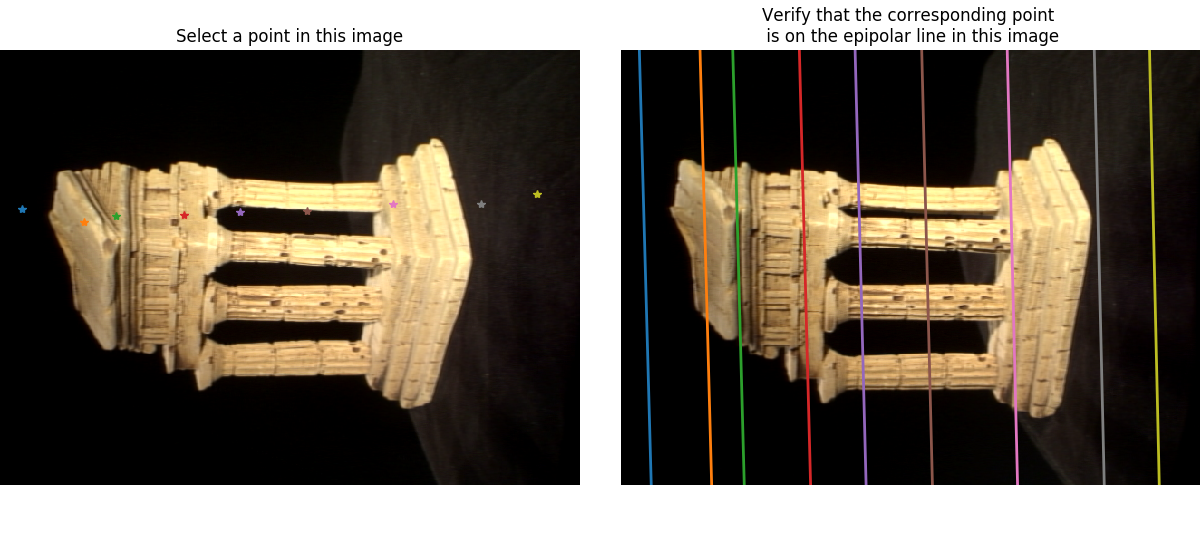
\includegraphics[width=\textwidth]{images/RANSAC.png}}
\end{tabular}
\caption{Seven-Point Algorithm with RANSAC Output}
\end{figure}

\subsection{Rodrigues Formula}
The formulae were implemented and verified with OpenCV's results as well.

\subsection{Optimization}

\begin{figure}[!ht]
\centering
\begin{BVerbatim}
Re-projection Error for all Noisy Points: 474443.6399674097
Re-projection Error for Inlier Points (Before Optimization): 306.2297910673943
Re-projection Error for Inlier Points (After Optimization): 7.742333732219369
\end{BVerbatim}
\caption{Re-projection Errors}
\end{figure}

\begin{figure}[!ht]
\centering
\begin{tabular}{ccc}
{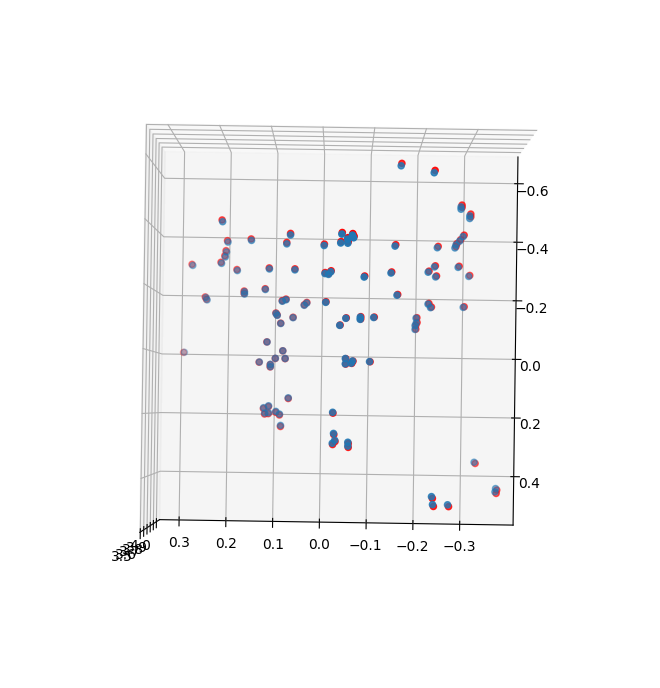
\includegraphics[width=0.3\textwidth]{images/ba_plot1.png}} &
{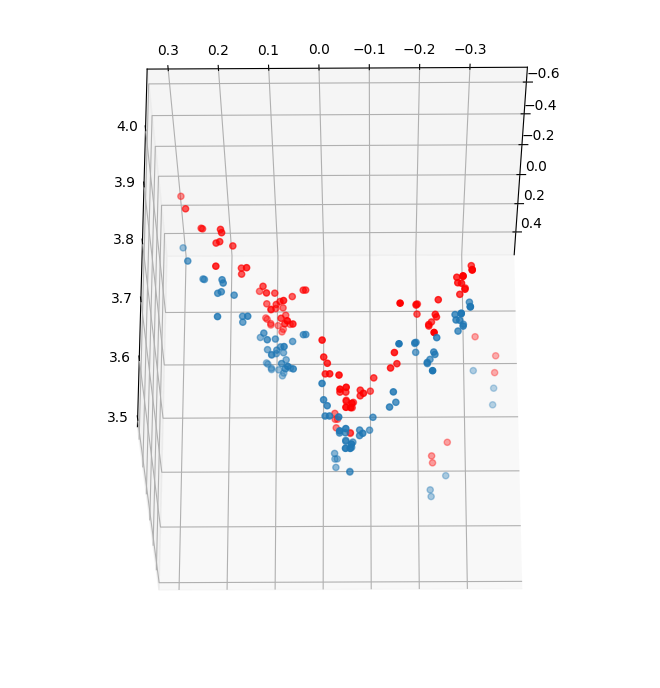
\includegraphics[width=0.3\textwidth]{images/ba_plot2.png}} &
{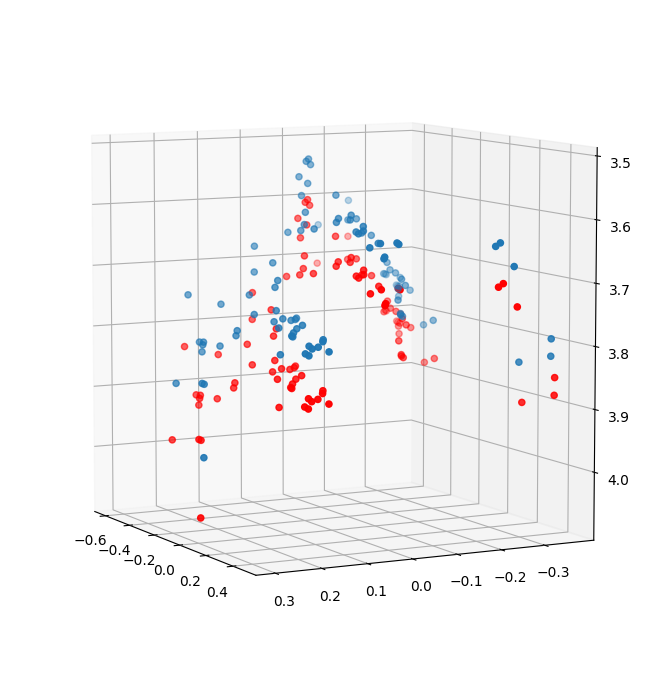
\includegraphics[width=0.3\textwidth]{images/ba_plot3.png}}
\end{tabular}
\caption{3D Visualization of the Points (Front, Top and Bottom views) (Red-Before, Blue-After)}
\end{figure}

\begin{figure}[!ht]
\centering
\begin{tabular}{c}
{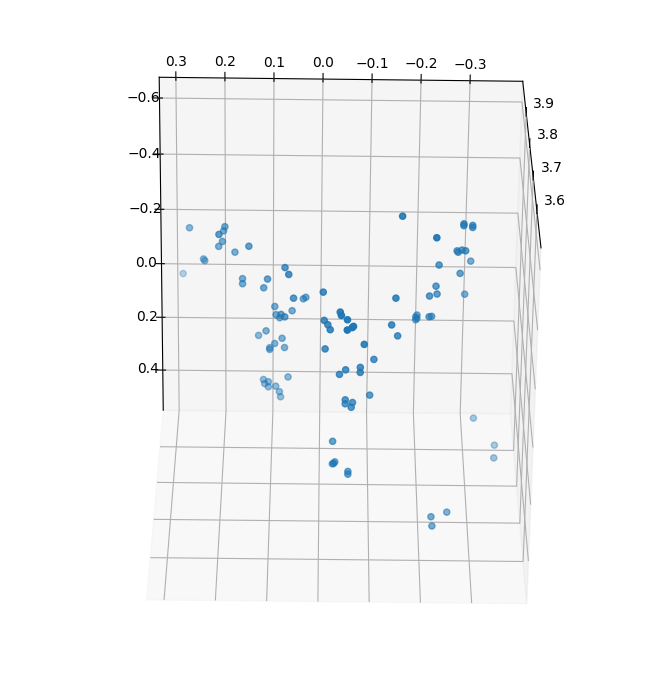
\includegraphics[width=0.9\textwidth]{images/ba1.png}}
\end{tabular}
\caption{3D Visualization of the Points after Optimization}
\end{figure}

\end{document} 